\section{(R)evolution!}


\slide{C++ is becoming more and more complicated...}{
    \centering
    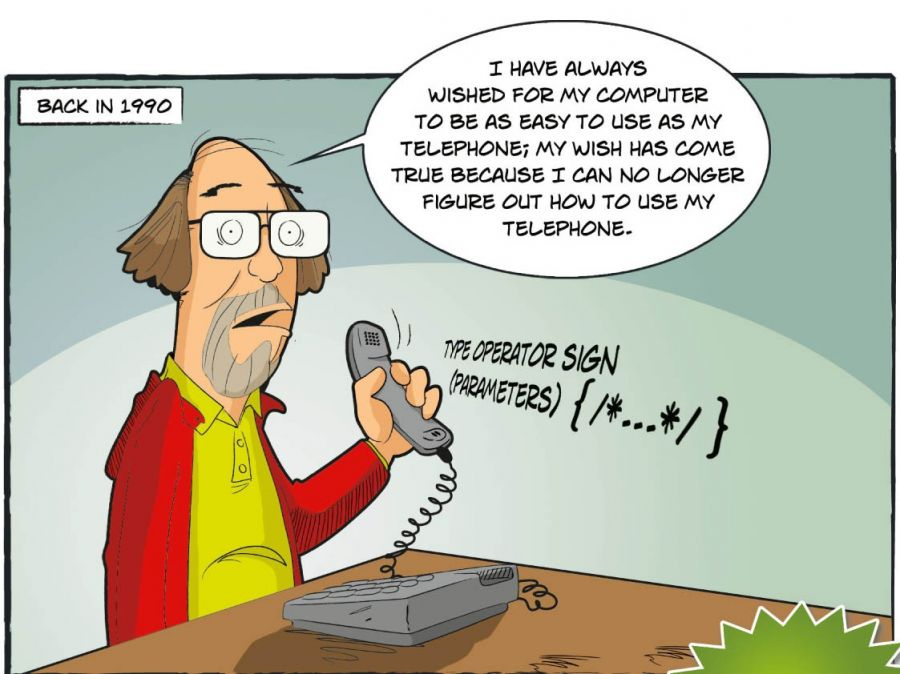
\includegraphics[height=0.8\paperheight]{bjarne-telephone}
}


\slide{(R)evolution!}{
    \centering
    \only<1>{\LARGE Evolution of C++ vs Revolution of C++}
    \only<2>{
\includegraphics[height=0.8\paperheight]{devolution}}
    \only<3>{
\includegraphics[height=0.8\paperheight]{your-cat-is-evolving}}
}


\slide{C++ standard implementation delays}{
    \begin{table}
        %\caption{C++ users}
        \begin{tabular}{|l|r|r|}
            \hline \textbf{Version} & \textbf{Standard} & \textbf{First implementation} \\
            \hline 
            \hline C84 & "the ARM" - 1989 & - \\
            \hline
            \hline C++98 & IX 1998 & 2003 (EDG + Dinkumware) \\
            \hline C++03 & X 2003 & gcc? \\
            \hline C++11 & IX 2011 & IV 2013 (clang3.3) \\
            \hline C++14 & III 2014 & XI 2013 (clang 3.4) \\
            \hline C++17 & ? & ? \\
            \hline
        \end{tabular}
    \end{table}
}


\slide{Free lunch is over}{
    \begin{columns}
    \begin{column}{0.57\textwidth}
        \begin{itemize}[<+->]
            \item Moore's law is no applicable anymore % Free lunch is over
            \item Processor speed doesn't rise
            \item We must go into cuncurrency
            \item We must write multithreded apps
            \item We must write efficient and effective code
            \item Modern C++ facilitate above needs % Effective modern C++
            \item VM languages will not be faster than C++
            \item More and more mobile apps are written in C++
            \item Can C perform better? % Basz
        \end{itemize}
    \end{column}
    \begin{column}{0.43\textwidth}
        \only<1-5>{\centering 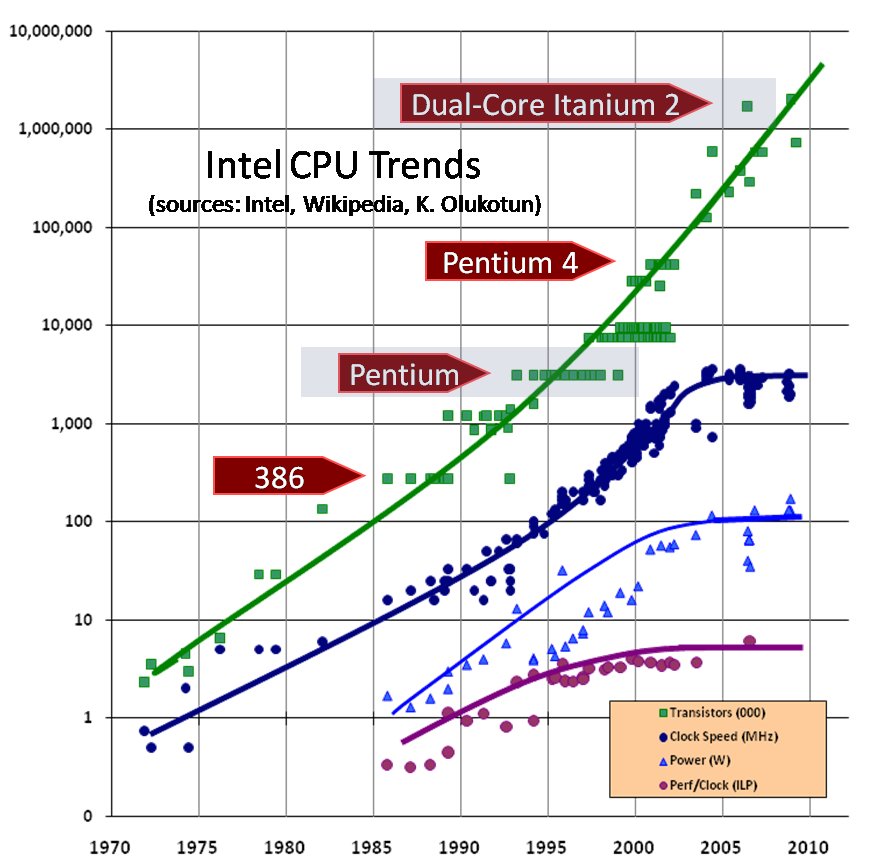
\includegraphics[height=0.6\paperheight]{free-lunch-is-over} \\
                   \scriptsize \url{http://www.gotw.ca/publications/concurrency-ddj.htm}}
        \only<6-8>{\centering 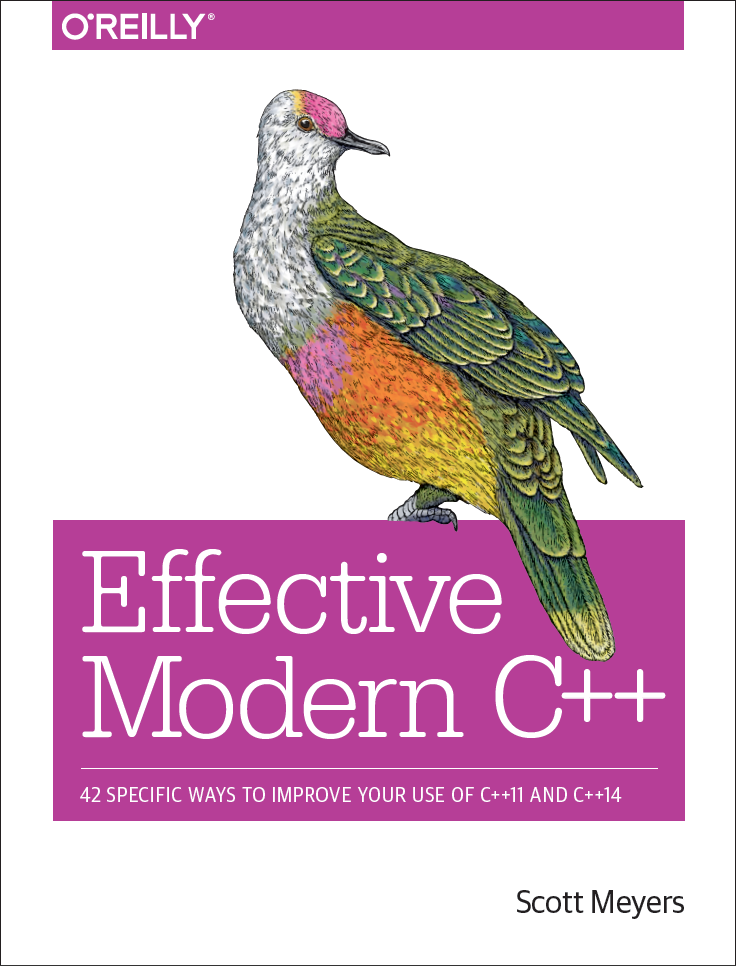
\includegraphics[height=0.7\paperheight]{effective-modern-cpp} \\
                   \scriptsize (This book cover is real)}
        \only<9>{\centering 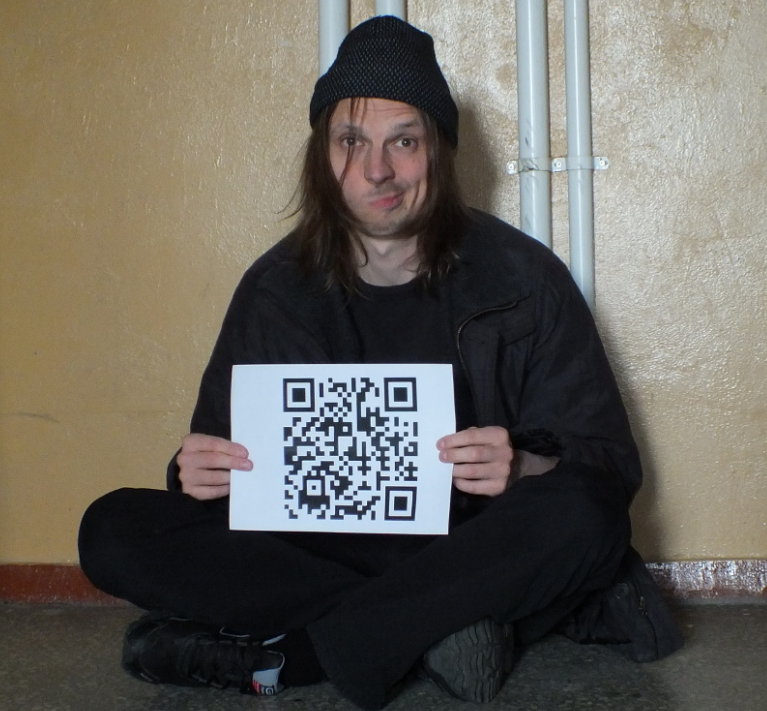
\includegraphics[height=0.6\paperheight]{szurgot} \\
                {\scriptsize Bartosz 'BaSz' Szurgot \\ C++ vs. C: The embedded perspective \\ code::dive 2015 }}
    \end{column}        
    \end{columns}
}